\documentclass{article}
\LARGE
% Language setting
% Replace `english' with e.g. `spanish' to change the document language
\usepackage[english]{babel}

% Set page size and margins
% Replace `letterpaper' with `a4paper' for UK/EU standard size
\usepackage[letterpaper,top=2cm,bottom=2cm,left=3cm,right=3cm,marginparwidth=1.75cm]{geometry}


\usepackage{tikz}
\usetikzlibrary{shapes.geometric, arrows}
\tikzstyle{startstop} = [rectangle, rounded corners, minimum width=3cm, minimum height=1cm,text centered, draw=black, fill=red!30]
\tikzstyle{io} = [trapezium, trapezium left angle=70, trapezium right angle=110, minimum width=3cm, minimum height=1cm, text centered, draw=black, fill=blue!30]
\tikzstyle{process} = [rectangle, minimum width=3cm, minimum height=1cm, text centered, draw=black, fill=orange!30]
\tikzstyle{decision} = [diamond, minimum width=3cm, minimum height=1cm, text centered, draw=black, fill=green!30]
\tikzstyle{arrow} = [thick,->,>=stealth]




\pgfdeclarelayer{bg}
\pgfsetlayers{bg,main}

% Useful packages
\usepackage{amsmath}
\usepackage{amsfonts}
\usepackage{graphicx}
\usepackage[colorlinks=true, allcolors=cyan]{hyperref}
\numberwithin{equation}{section}
\usepackage{graphicx,wrapfig,lipsum,subfigure,sidecap,epsfig}
\usepackage{caption}
\usepackage{cancel}
%\usepackage{graphicx,subfigure,sidecap,epsfig} % Rouslan's subfig package
\usepackage{soul}
%\usepackage[colorlinks=true,linkcolor=red]{hyperref}%
\usepackage{mathtools}
\usepackage{eqparbox}
\usepackage{float} % \figure{}[H] IN PLACE VIEW
\usepackage[capitalize]{cleveref} % smart references in one bracket
\usepackage{hyperref}
\usepackage{amssymb} % rightleft arrows
\usepackage{cancel} % \cancelto{<value>}{expression} diagonally
\usepackage[mathscr]{euscript}
\DeclareSymbolFont{rsfs}{U}{rsfs}{m}{n}
\DeclareSymbolFontAlphabet{\mathscrsfs}{rsfs}
\usepackage{MnSymbol}


%
% CREF rules
% Equation(s)
\crefformat{equation}{#2Eq. (#1)#3}
\crefrangeformat{equation}{#3Eqs. (#1)#4 to #5(#2)#6}
\crefmultiformat{equation}{#2Eqs. (#1)#3}{ and #2(#1)#3}{, #2(#1)#3}{ and #2(#1)#3}
\crefrangemultiformat{equation}{#3Eqs. ((#1))#4 to #5((#2))#6}{ and #3(#1)#4 to #5(#2)#6}{, #3(#1)#4 to #5(#2)#6}{ and #3(#1)#4 to #5(#2)#6}
% Plural eqn
\crefformat{pluralequation}{#2Eqs.~(#1)#3}
% System
\crefformat{system}{#2Sys.~(#1)#3}
\crefrangeformat{system}{#3Sys. (#1)#4 to #5(#2)#6}
\crefmultiformat{system}{#2Sys. (#1)#3}{ and #2(#1)#3}{, #2(#1)#3}{ and #2(#1)#3}
\crefrangemultiformat{system}{#3Sys. ((#1))#4 to #5((#2))#6}{ and #3(#1)#4 to #5(#2)#6}{, #3(#1)#4 to #5(#2)#6}{ and #3(#1)#4 to #5(#2)#6}
% Boundary conditions
\crefformat{bc}{#2BC (#1)#3}
\crefrangeformat{bc}{#3BCs (#1)#4 to #5(#2)#6}
\crefmultiformat{bc}{#2BCs (#1)#3}{ and #2(#1)#3}{, #2(#1)#3}{ and #2(#1)#3}
\crefrangemultiformat{bc}{#3BCs ((#1))#4 to #5((#2))#6}{ and #3(#1)#4 to #5(#2)#6}{, #3(#1)#4 to #5(#2)#6}{ and #3(#1)#4 to #5(#2)#6}
% Steps
\crefformat{step}{#2Step (#1)#3}
\crefrangeformat{step}{#3Steps (#1)#4 to #5(#2)#6}
\crefmultiformat{step}{#2Steps (#1)#3}{ and #2(#1)#3}{, #2(#1)#3}{ and #2(#1)#3}
\crefrangemultiformat{step}{#3Steps ((#1))#4 to #5((#2))#6}{ and #3(#1)#4 to #5(#2)#6}{, #3(#1)#4 to #5(#2)#6}{ and #3(#1)#4 to #5(#2)#6}
%diagram
\crefformat{diagram}{#2Diagram (#1)#3}
\crefrangeformat{diagram}{#3Diagrams (#1)#4 to #5(#2)#6}
\crefmultiformat{diagram}{#2Diagrams (#1)#3}{ and #2(#1)#3}{, #2(#1)#3}{ and #2(#1)#3}
\crefrangemultiformat{diagram}{#3Diagrams ((#1))#4 to #5((#2))#6}{ and #3(#1)#4 to #5(#2)#6}{, #3(#1)#4 to #5(#2)#6}{ and #3(#1)#4 to #5(#2)#6}



%\usepackage[sortcites=true]{biblatex} % biblatex DOEST WORK WITH LIVE TYPESETTER
\usepackage[nocompress]{cite}
%\bibliographystyle{ieeetr} % trash style mess up the order in bib

\graphicspath{{figures/}}


%%% Todos
\newcommand{\todo}[1]{\vspace{5 mm}\par \noindent
\marginpar{\textsc{\tiny \hspace{0.5cm} ToDo}} \framebox{\begin{minipage}[c]{0.95
\textwidth} \small \tt #1 \end{minipage}}\vspace{5 mm}\par}



\title{Discrete stream function method \\ for the incompressible Navier-Stokes equations \\with simple boundary conditions}
\author{Rauan}

\begin{document}
\maketitle

\begin{abstract}
The goal of these notes is to present the detailed overview of discrete stream function method for solving incompressible Navier-Stokes equations with simple boundary conditions. We will discuss in detail the scheme formulation, transient and spatial discretizations. Special attention will be paid to the change of unknown variables. After studying these notes one must get a coherent picture of the application of discrete stream function method to incompressible flows with simple Boundary Conditions (BCs) and be able to implement the scheme in code.
\end{abstract}

\tableofcontents

\section{Introduction}\label{sec:introduction}

In these notes we will be concerned with the discretization of the Navier-Stokes equations describing the flow of an incompressible fluid past the 2-dimensional cylinder with a singular boundary force f added to the momentum equation as a continuous analog of the immersed boundary formulation:
\begin{subequations}
\label[pluralequation]{eqs:NSE}
\begin{align}
\label{eqn:momentum-intro}
\frac{\partial \boldsymbol{v}}{\partial t} + \boldsymbol{v} \cdot \nabla \boldsymbol{v} &= -\nabla p + \epsilon \nabla \cdot \nabla \boldsymbol{v} +\int_{s}\boldsymbol{f}(\xi(s,t))\delta(\xi-x)ds\\
\label{eqn:continuity}
\nabla \cdot \boldsymbol{v} &= 0,\\
\boldsymbol{v}(\xi(s,t)) &= \int_x\boldsymbol{v}(x)\delta(x - \xi)dx = \boldsymbol{v}_B(\xi(x,t)),
\end{align}
\end{subequations}
which are written here in the non-dimensional form, i.e. $\epsilon \equiv Re^{-1}$ for brevity; also $\boldsymbol{v}$ is the velocity and $p$ pressure fields. The boundary conditions are assumed to be simple, i.e.  Dirichlet and Neumann for the normal and tangential velocities, respectively. Spatial variable $x$ represents position in the flow field, $\mathscrsfs{D}$, and $\xi$ denotes coordinates along the immersed boundary, $\partial \mathscrsfs{B}$ having a velocity of $\boldsymbol{v}_B$. The geometry of the immersed object $\mathscrsfs{B}$ is considered to be of arbitrary shape. 
\begin{figure}[H] % here - h, bottom - b, top - t
  \centering{
  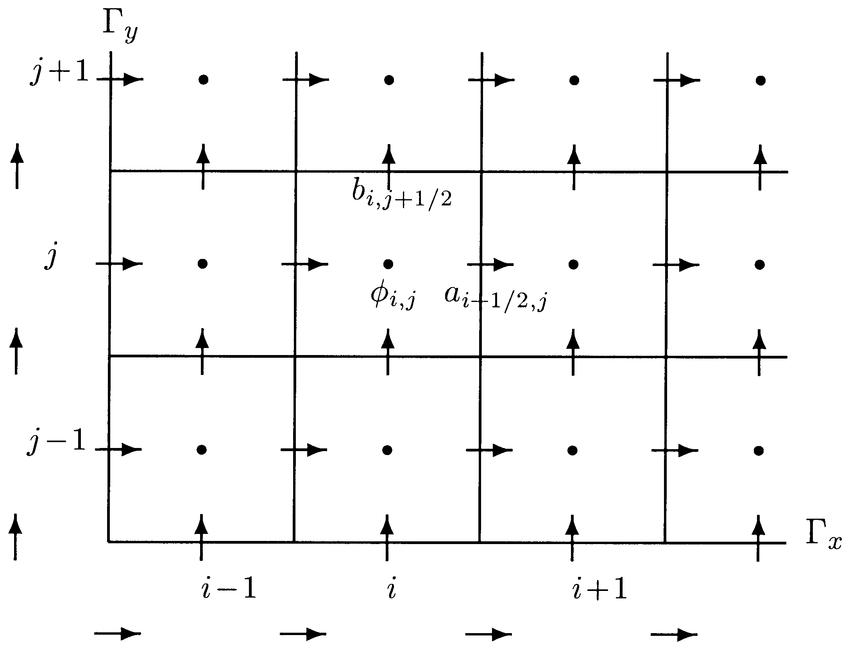
\includegraphics[width=0.55\paperwidth]{fig1}
  }
  \caption{Staggered grid discretization of a two-dimensional computational domain $\mathscrsfs{D}$ and immersed boundary formulation for a body $\mathscrsfs{B}$ depicted by a shaded object. The horizontal and vertical arrows ($\rightarrow$, $\uparrow$) represent the discrete $u_i$ and $v_i$ velocity components, respectively. Pressure $p_i$ is positioned at the center of each cell ($\times$). Lagrangian points, $\xi_k$ = ($\xi_k$, $\eta_k$), along $\partial\mathscrsfs{B}$ are shown with filled squares ($\filledsquare$) where boundary forces $\boldsymbol{f}_k=(f_{x,k},f_{y,k})$ are applied ($\Rightarrow,\Uparrow$).}\label{fig:1}
\end{figure}

The above system is discretized with a standard staggered Cartesian grid finite volume method. The mesh and variable locations are depicted in \cref{fig:1}. The computational domain, $\mathscrsfs{D}$, is represented by a Cartesian grid, ($x_i, y_i$), and the immersed boundary, $\mathscrsfs{B}$ is described by a set of Lagrangian points, ($\xi_k,\eta_k$), which can be a function of time.

\section{Discretization}\label{sec:discretization}

We can rewrite \cref{eqs:NSE} using discrete differential operators as 
\begin{equation}\label[pluralequation]{eqs:discrete-nse}
\begin{aligned}
	M\frac{dq}{dt} + Gp - Hf &= \mathbf{N}(q) + Lq + bc_1&\text{ (momentum),}\\
	Dq &= 0 + bc_2&\text{ (continuity),}\\
	Eq & = \boldsymbol{v}_B^{n+1} &\text{ (no-slip condition),}
	\end{aligned}
\end{equation}
where $q=(  u\Delta y,v\Delta x )$, $p$ and $f$ are the discrete velocity flux vector, pressure, and boundary force. Discretized non-linear advective term $\boldsymbol{v}\cdot\nabla \boldsymbol{v}$ is denoted as $\mathbb{N}(q)$, whereas operators $M$,$L$ are mass matrix and discrete Laplacian respectively. Operators $G$ and $D$ are discrete gradient and divergence matrices s.t. $D=-G^T$ and \cite{Chang:2002,Perot:1993}. The rest operators $E$ and $H$ are the interpolation and regularization operators resulting from the regularization of the Dirac delta functions in momentum and no-slip equations, which are constructed in such a way that $E=-H^T$. No-slip constraint is enforced by equating the boundary velocity, $\boldsymbol{v}_B$, to the velocity value along $\partial \mathscrsfs{B}$ interpolated by $E$ from the neighbouring cells. Regularization operator diffuses the singular boundary force along $\partial \mathscrsfs{B}$ to the Cartesian grid \cite{Colonius:2008}.  \cref{eqs:discrete-nse} are represented as system of linear equations
\begin{equation}\label[system]{sys:discrete-penult-nse}
	\begin{bmatrix}{}
  A & G & -H \\
  D& 0& 0\\
  E & 0 & 0
\end{bmatrix}
\begin{pmatrix}{}
	q \\
	p \\
  	f
\end{pmatrix}=
\begin{pmatrix}{}
	r^{n} \\
	0 \\
  	\boldsymbol{v}_B^{n+1}
\end{pmatrix}
+\begin{pmatrix}{}
	bc_1 \\
	bc_2 \\
  	0
\end{pmatrix},
\end{equation}
where $A = \frac{1}{\Delta t} M - \frac{1}{2} L$ comes from implicit treatment using trapezoid method of viscous terms. Explicit term $r^n=\left( \frac{1}{\Delta t}M + \frac{1}{2} L\right)q^n + \frac{3}{2}\mathbb{N}(q^n) - \frac{1}{2}\mathbf{N}(q^{n-1})$ is also obtained from applying Adams-Bashforth scheme to advective term. We can use the properties of operators discussed above to rewrite \cref{sys:discrete-penult-nse} as 
\begin{equation}\label[system]{sys:discrete-nse}
	\begin{bmatrix}{}
  A & G & E^T \\
  G^T& 0& 0\\
  E & 0 & 0
\end{bmatrix}
\begin{pmatrix}{}
	q \\
	p \\
  	\tilde{f}
\end{pmatrix}=
\begin{pmatrix}{}
	r^{n} \\
	0 \\
  	\boldsymbol{v}_B^{n+1}
\end{pmatrix}
+\begin{pmatrix}{}
	bc_1 \\
	-bc_2 \\
  	0
\end{pmatrix},
\end{equation}
making the above system of linear algebraic equations symmetric. 
	Here, $\tilde{f}$ is the boundary force with an incorporated scaling factor. This form of the equation is known as the Karush–Kahn–Tucker (KKT) system where $(p,\tilde{f})^T$ appear as a set of Lagrange multiplier to satisfy a set of kinematic constraints. In the discretized set of equations, the constraints are purely numerical and it is no longer necessary to distinguish the pressure and boundary force. Instead we can define a combined variable $\lambda = (p,\tilde{f})^T$ for the Lagrange multipliers and group the submatrices as $Q = [G, E^T]$. Note that by removing the boundary force and no-slip condition along $\partial \mathscrsfs{B}$, the traditional discretization of the incompressible Navier–Stokes equations can be retrieved, i.e. being equivalent to applying divergence to momentum and obtaining pressure-Poisson.

Next, we apply the classical projection (fractional-step) algorithm to \cref{{sys:discrete-nse}}, which can be expressed as an approximate $LU$ decomposition of the left-hand side matrix, to produce the immersed boundary projection method \cite{Colonius:2008}:
\begin{enumerate}
	\item $A q^*=r_1, \quad$ (Solve for intermediate velocity).
	\item $Q^{\mathrm{T}} A_j^{\dagger} Q \lambda=Q^{\mathrm{T}} q^*-r_2, \quad$ (Solve a modified Poisson equation).
	\item $q^{n+1}=q^*-A_j^{\dagger} Q \lambda, \quad$(Projection step).
\end{enumerate}
Here $A^{\dagger}_{j}$ denotes the $j$-th order Taylor series expansion of $A^{-1}$ with respect to $\Delta t$. The explicit terms on the right-hand side have been grouped into $r_1$ and $r_2$. Matrices $A$ and $Q^TA^\dagger_jQ$ are constructed to be symmetric positive definite operators in order to use the conjugate-gradient method to efficiently solve for the intermediate velocity and the Lagrange multipliers. All boundary conditions are set to uniform flow $(U_{\infty}, 0, 0)$ in the streamwise direction ($x$-direction) except for the outflow boundary where a convective boundary condition:
\begin{equation}
  \frac{\partial\boldsymbol{v}}{\partial t} + U_\infty \frac{\partial \boldsymbol{v}}{\partial x}=0
\end{equation}




	
\section{Summary}\label{sec:summary}
	

\pagebreak
\bibliographystyle{plain}
\bibliography{Zotero.bib}
 

\pagebreak
\appendix
\section{Appendix}

\subsection{Transient schemes}

\end{document}
